\chapter{Use Cases} \label{ch:usecases}

To guide and simplify the interactive exploration of the SDG, the \SB implements four concrete \emph{use cases}, which 
were briefly explained in \autoref{sec:intro-tool} already. Those use cases were identified by Keba engineers to 
provide potentially helpful insights when investigating the code, trying to fix certain problems, or when making 
changes. This chapter will give a description of each of the four use cases (\emph{Executions}, \emph{Variable 
Assignment}, \emph{Change Impact}, and \emph{Change Cause}) and illustrate them with examples.

A use case in this context is basically a strategy for deciding which parts of the whole SDG should be presented to the 
user, together with a set of element types which are valid \emph{targets} (starting points) it can apply to (e.g.\ 
statements, variables, procedures). The \emph{result} of a use case is that part of the SDG which would be visible to 
the user if they were to expand every node in the graph (similar to a \emph{slice} of the 
program~\cite{DBLP:journals/tse/Weiser84}).

The \SB implements use cases in a modular way, which makes it easy to add new ones or add custom behavior to existing 
ones. See \autoref{ch:impl} for a detailed description on that.


\section{Executions}

The targets of this use case are executable elements, i.e.\ statements and procedures. The goal is to find out how 
a statement or procedure can be executed, that is, which execution paths in the program may lead to it being executed. 
The result is a graph of all possible stack traces one could observe for the target, but also including conditional 
statements between calls.

\autoref{fig:sdg-executions_one} shows an example for the Executions of the highlighted statement for one particular 
object instance (source code in \autoref{lst:sdg-instances}, \autopageref{lst:sdg-instances}). The nodes and edges in 
the SDG which are not part of the result (i.e.\ will not be displayed) are grayed out. \autoref{fig:sdg-executions_all} 
shows the same example for all instances of the statement (now grouped by a \emph{dummy node}), which is usually the 
result when a statement is selected in the source code.

The resulting graph contains all nodes the target is directly or indirectly control-dependent on. Those nodes are found 
by including all predecessor nodes which connect via a control edge to any node already in the graph. In figures 
\ref{fig:sdg-executions_one} and \ref{fig:sdg-executions_all} we can see that the highlighted target statement depends 
on the execution of the respective procedure containing it, which in turn depends on one or more activation nodes (this 
means the procedure will be executed only if any activation node is executed). The activation nodes then depend on the 
respective statement containing the call, which in turn depend on their containing procedure, \lstinline|main| in this 
case.

\begin{figure}[tbp]
  \centering
    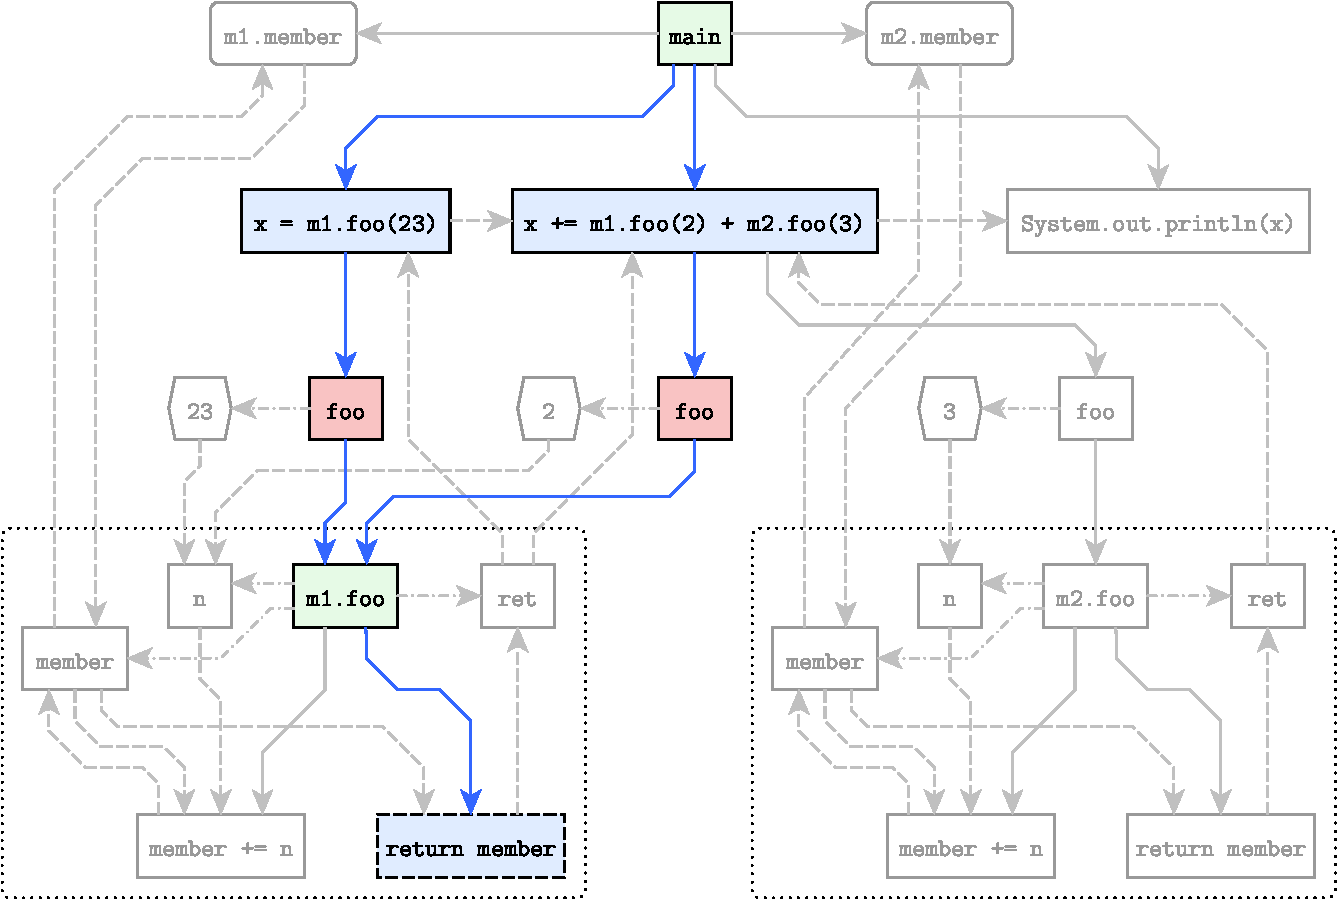
\includegraphics[scale=0.6]{sdgs/executions_one}
  \caption{Executions for one instance of a statement}
  \label{fig:sdg-executions_one}
\end{figure}

\begin{figure}[tbp]
  \centering
    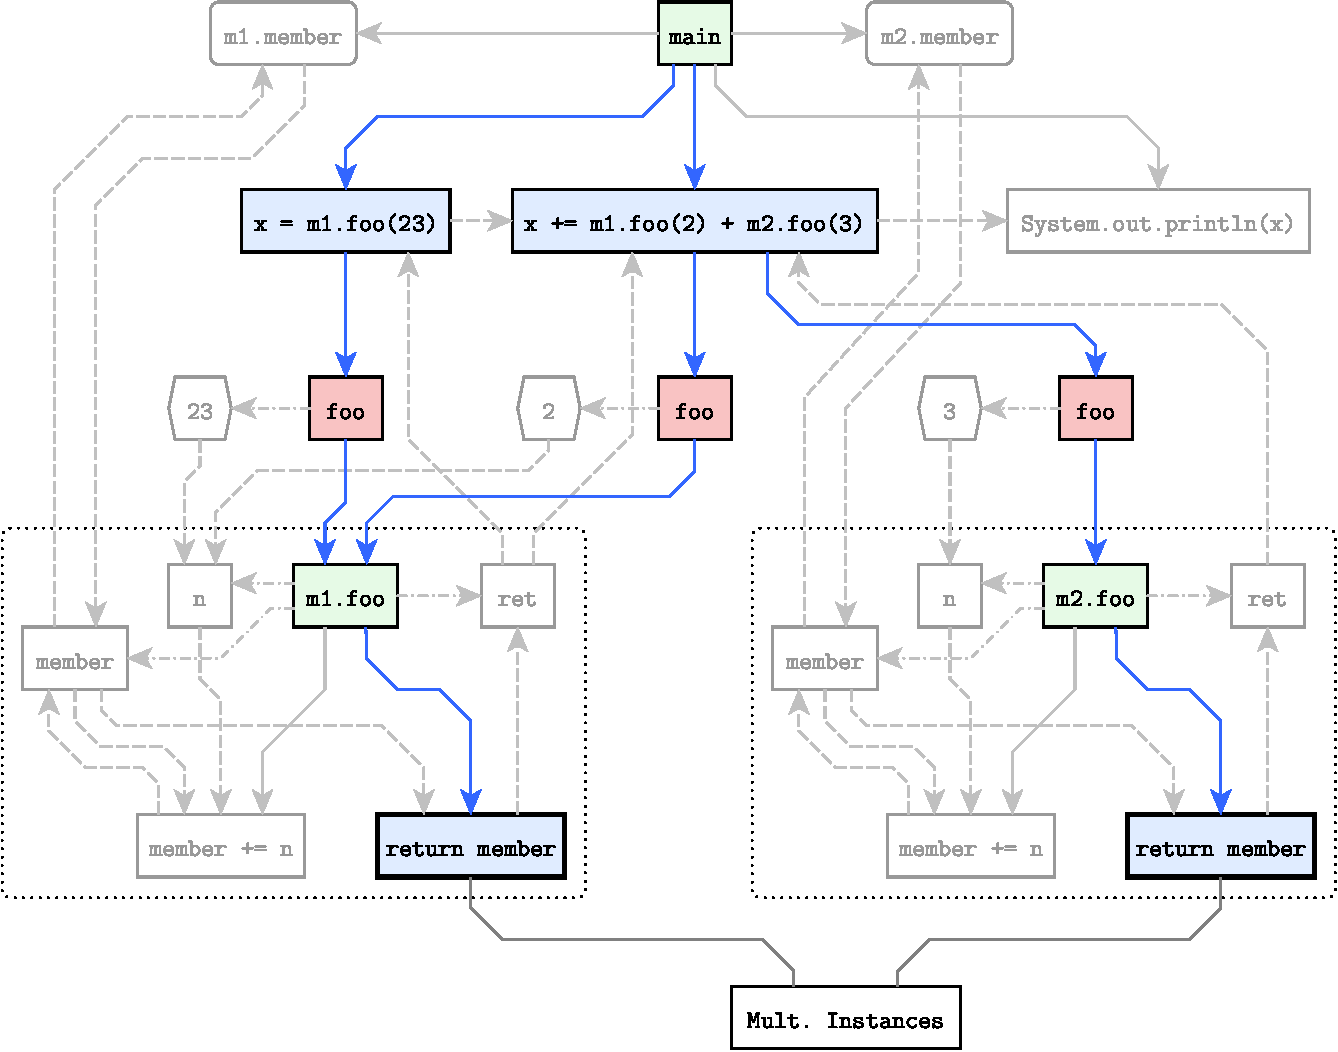
\includegraphics[scale=0.6]{sdgs/executions_all}
  \caption{Executions for all instances of a statement, grouped by a dummy node}
  \label{fig:sdg-executions_all}
\end{figure}


\section{Variable Assignment}

The targets of this use case are variables of any kind (global, member, and local variables; formal parameters). The 
goal is to find out which sequences of statements could cause a variable to change its value. The result is a graph 
that contains the variable node (which may be an artificial node in case of a local variable), all statements directly 
writing to that variable, and for those statements their \emph{Executions}.

\autoref{fig:sdg-assignment_one} shows an example for the Variable Assignment of the highlighted instance of a member 
variable (source code in \autoref{lst:sdg-instances}, \autopageref{lst:sdg-instances}). There is one statement that 
writes to the variable, connected via an incoming data edge. Note that the formal parameter node for the member 
variable is not displayed, instead an artificial edge is added directly from the writing statement to the variable 
node. The rest of the graph is the same as for the \emph{Executions} for that writing statement, i.e.\ statements and 
procedures which the statement is control-dependent on.

\begin{figure}[htbp]
  \centering
    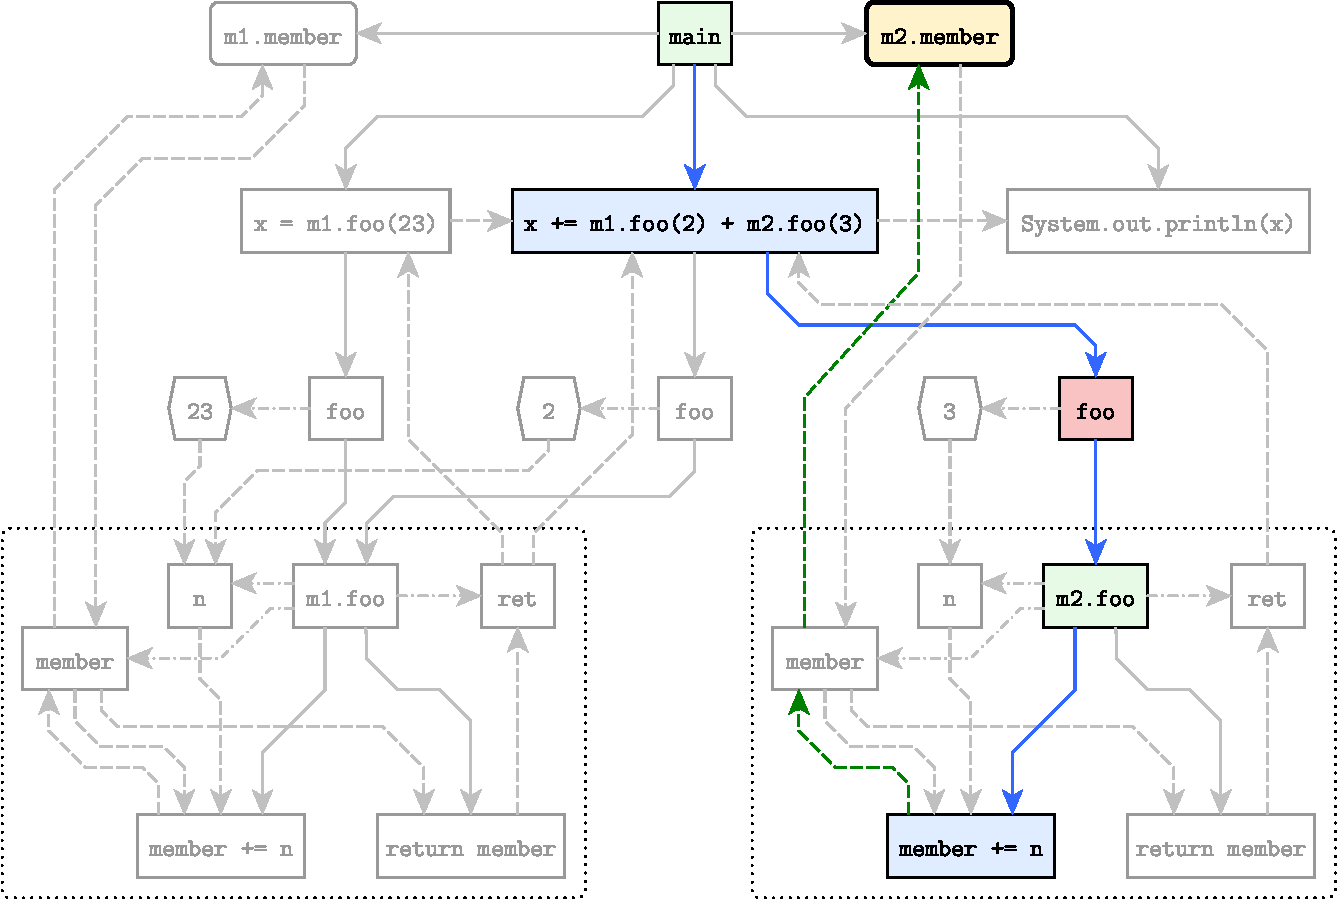
\includegraphics[scale=0.6]{sdgs/assignment_one}
  \caption{Variable Assignment for one instance of a member variable}
  \label{fig:sdg-assignment_one}
\end{figure}

For variables that are represented in the SDG (member and global variables, parameters to procedures), constructing the 
graph for this use case is straight forward: just find predecessors which are statement nodes connected via data edges 
(possibly ignoring intermediate formal parameter nodes), and from there continue as for \emph{Executions}. Local 
variables, on the other hand, are not represented in the SDG. To be able to include local variables as well, the \SB 
introduces an artificial node representing the local variable for each instance of the procedure declaring it. The AST 
is then searched for each assignment, or use as a reference or output parameter, of the variable. From the resulting 
AST nodes the corresponding statement nodes in the SDG are found and connected to the artificial node via synthetic 
data edges.


\section{Change Impact}

This use case targets all nodes in the SDG. The goal is to find all statements and variables which might be influenced 
(whether a statement or procedure is executed; changes to a variable's value). The result is a graph which contains all 
nodes directly or indirectly influenced by the execution of a statement or procedure, or by a variable's value.

The example in \autoref{fig:sdg-changeimpact} shows a change impact for the highlighted return statement (source code 
in \autoref{lst:sdg-calls}, \autopageref{lst:sdg-calls}). The return statement directly influences the procedure's 
return value, which in turn influences the value of variable \lstinline|res2| and the print statement (via the 
highlighted edges). Execution of the statement \lstinline|res2 = bar(res1)| influences the execution of procedure 
\lstinline|bar| (via the corresponding activation node). The value of parameter \lstinline|b| depends on the value of 
\lstinline|res2| and influences the execution of the conditional statement, which in turn determines which of the 
return statements get executed.

The change impact excludes certain edges, such as control edges from procedure nodes to their parameters, because 
parameters should not be included if they don't have any incoming data edges. Also excluded are any outgoing edges from 
the main procedure (which connects to all global and member variables, but doesn't actually influence their values).

We can see in the example that the return statement actually only influences the return value, which in turn influences 
the value of variable \lstinline|res2| and the print statement (via the highlighted edges). The change impact, however, 
also contains a lot of unrelated nodes, which is caused by the \SB following all outgoing data and control edges, 
regardless of whether they are actually influenced by incoming edges. In this example, the statement influenced by the 
return value of method \lstinline|bar| is not a conditional statement, so we know that the outgoing control edge is not 
influenced by the incoming data edge. The SDG, however, does not encode this kind of information.

This issue with change impacts is caused in part by the \SB itself, in part by the SDG. The \SB already has information 
on whether a statement is a conditional statement or not (because they are drawn differently), which could be used to 
exclude certain control edges from the change impact. It is, however, unknown at the time a node is expanded by the 
user whether or not there will be any incoming control edges from other nodes, so just filtering such control edges 
unconditionally is not an option.

\begin{figure}[htbp]
  \centering
    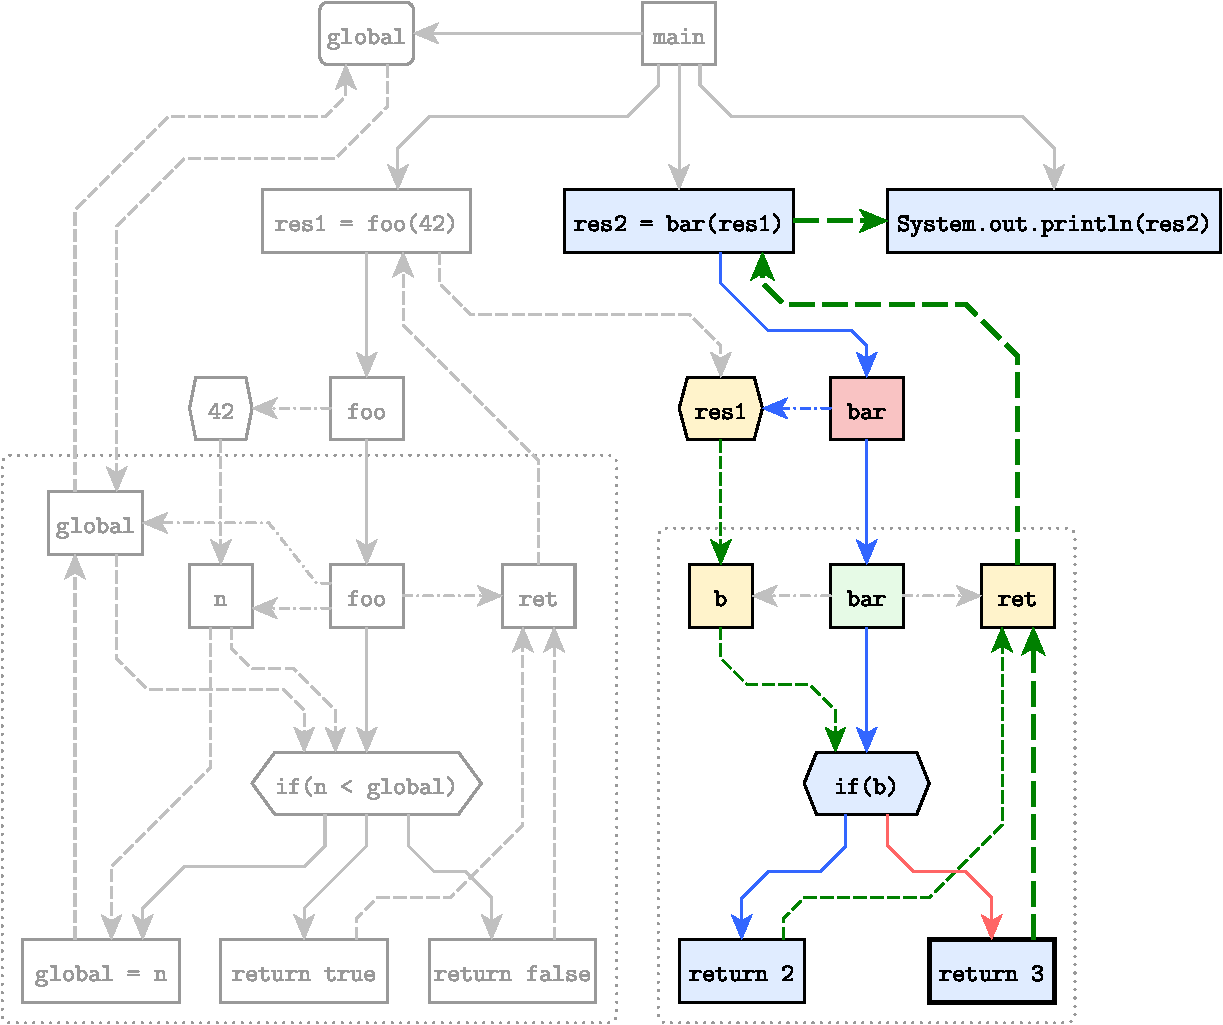
\includegraphics[scale=0.6]{sdgs/changeimpact}
  \caption{Change Impact for a return statement}
  \label{fig:sdg-changeimpact}
\end{figure}

%\begin{figure}[hp]
%  \centering
%    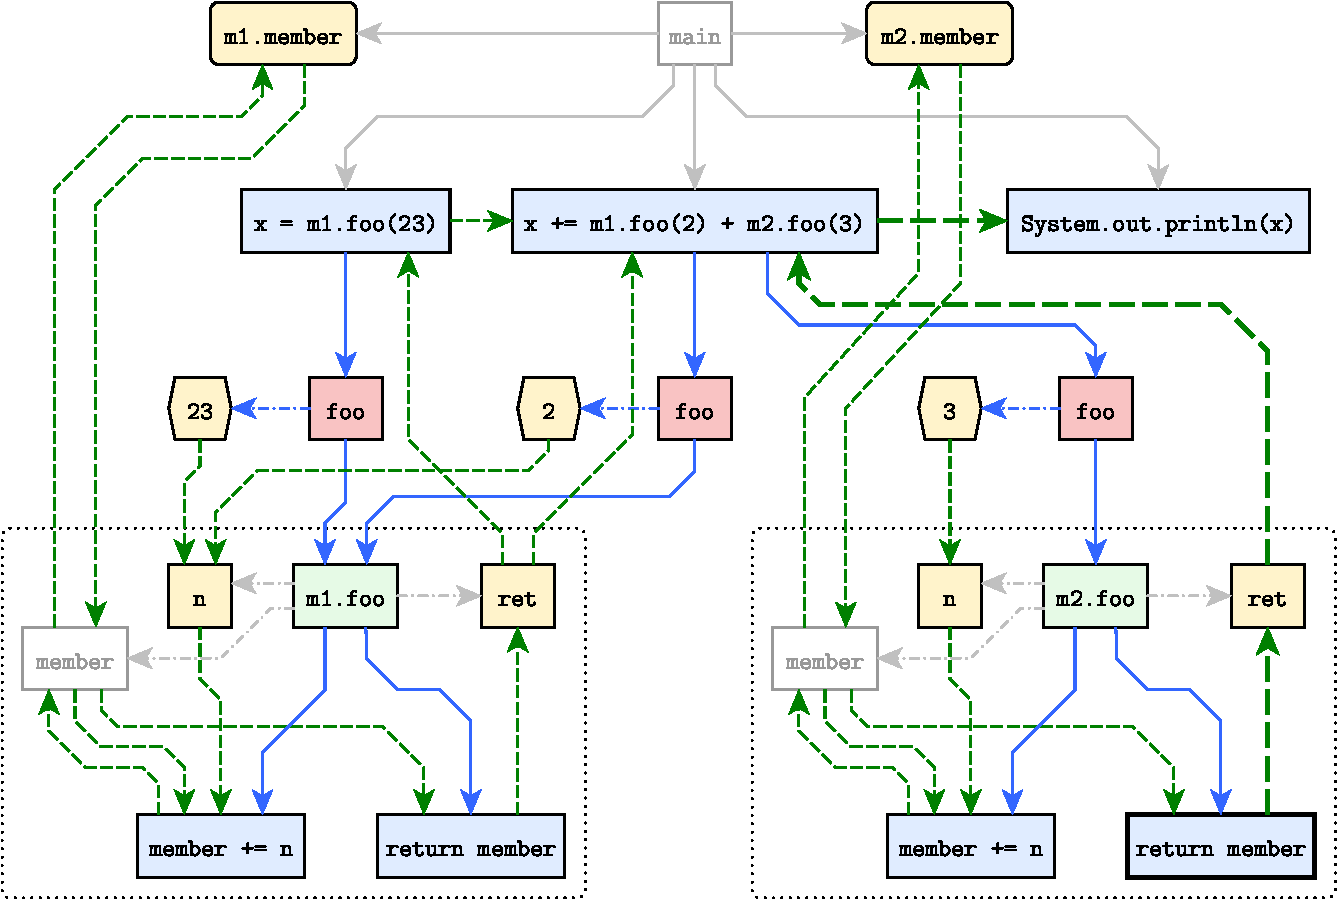
\includegraphics[scale=0.6]{sdgs/changeimpact2}
%  \caption{Change Impact showing a lot of unrelated nodes being included}
%  \label{fig:sdg-changeimpact2}
%\end{figure}


\section{Change Cause}

This use case is basically an inverse \emph{Change Impact}. It again targets all nodes in the SDG, the goal this time 
being to find all statements and variables which might influence the value of a variable or whether a statement gets 
executed. The result, therefore, is a graph which contains alls nodes directly or indirectly influencing the target 
node.

The example in \autoref{fig:sdg-changecause} shows a change cause for the highlighted assignment statement (source code 
in \autoref{lst:sdg-calls}, \autopageref{lst:sdg-calls}). The statement is directly influenced by the conditional, 
because it only gets executed if the conditional yields \lstinline|false|, and of course by the parameter which is 
assigned from. The conditional statement in turn depends on the value of the global variable and the parameter, as well 
as the execution of procedure \lstinline|foo|. The value of the formal parameter depends on the actual parameter, both 
are only relevant if their procedure or activation node, respectively, gets executed. Note that, as in the 
\emph{Variable Assignment} example, the formal parameter node for the global variable is not displayed, instead an 
artificial edge is added directly from the variable node to the reading statement.

\begin{figure}[htbp]
  \centering
    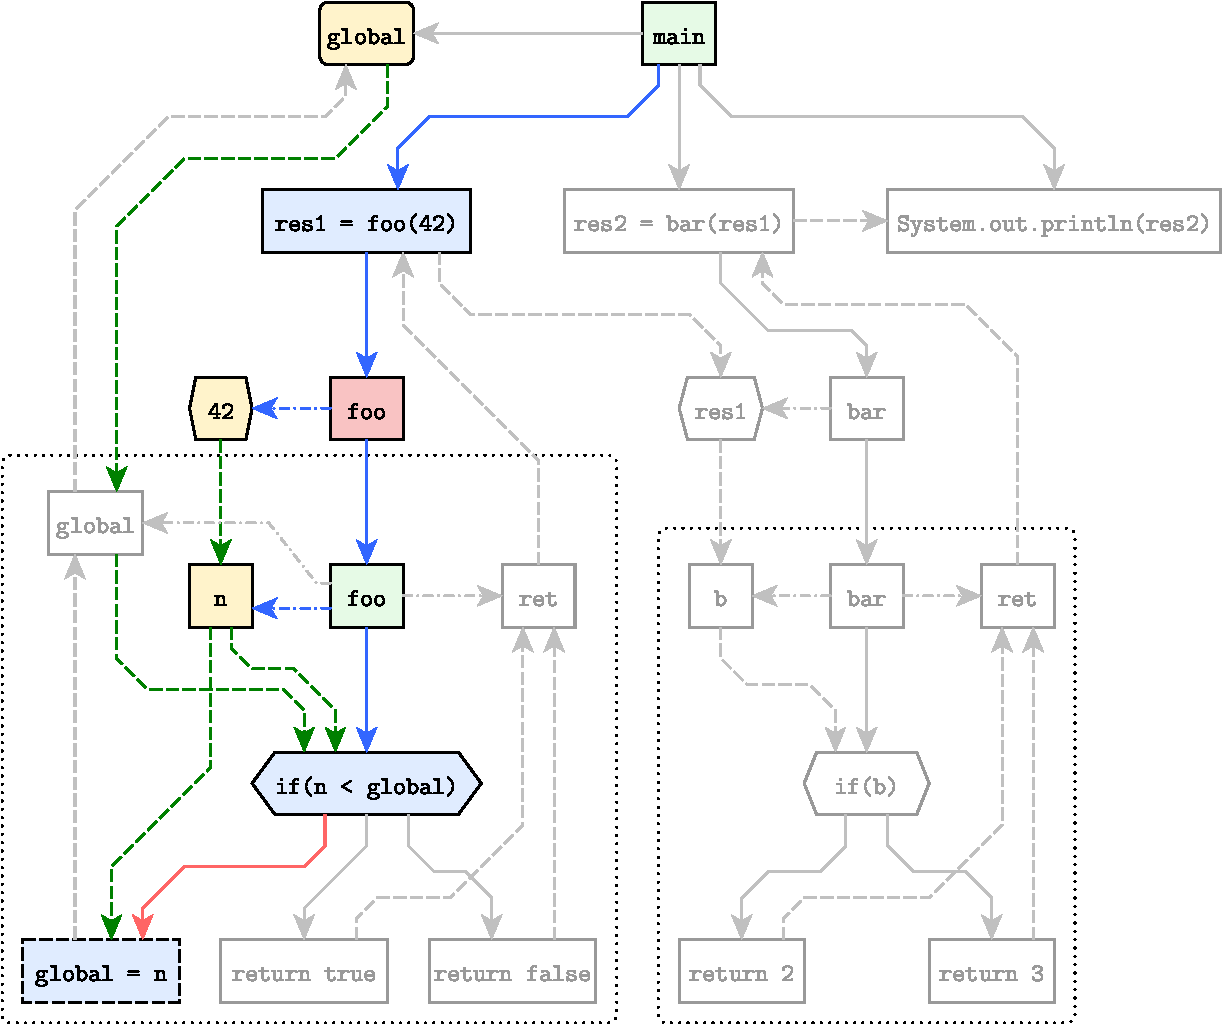
\includegraphics[scale=0.6]{sdgs/changecause}
  \caption{Change Cause for an assignment}
  \label{fig:sdg-changecause}
\end{figure}
